\documentclass{beamer}

\usetheme{Darmstadt}

\usepackage{graphics,xcolor}
\usepackage{graphicx}

% \usepackage{stmaryrd,amssymb,amsmath}

\newcommand{\nat}{\mathbb{N}}
\newcommand{\ints}{\mathbb{Z}}
\newcommand{\intersection}{\ensuremath{\cap}}
\newcommand {\emptyword}{\ensuremath{\epsilon}}
\newcommand {\len}[1] {\ensuremath{|#1|}}
\newcommand {\union} {\ensuremath{\cup}}



\begin{document}

\section{Established Results}



\begin{frame}
\frametitle{Unary finite automata}
Below, H(n) represents the function  $e^{\sqrt{nlog(n)}}$\\
\medskip
These are some statements related to unary finite automata
\medskip


\begin{itemize}
\item Each unary n-state 2dfa can be simulated by a 1dfa with O(H(n)) states.
\item For each n there is a unary n-state 2dfa A such that each 1dfa recognizing L(A) requires $\Omega$(H(n)) states.
\end{itemize}

\end{frame}




\begin{frame}
\frametitle{Unary finite automata}

 
\begin{itemize}
\item
For each n there is a unary n-state 2dfa A such that each 1nfa recognizing L(A) requires $\Omega$(H(n))
\item
Each unary n-state 1nfa A can be simulated by a 2dfa B with O($n^2$) states.
\item
For each n there is a unary n-state 1nfa A such that each 2dfa recognizing L(A) requires $\Omega$($n^2)$ states.
\end{itemize}

\end{frame}
\begin{frame}
\frametitle{Unary finite automata}
Informally speaking we can see that 2dfa's are hard to simulate by ldfa's, even if we consider only unary languages.\\
\medskip
Also, for unary languages,two-way motion is more powerful, in a sense, because we can simulate unary lnfa's by 2dfa's increasing the number of states only polynomially, which is not possible the other way round. 
\end{frame}
\begin{frame}
\frametitle{Unary finite automata}
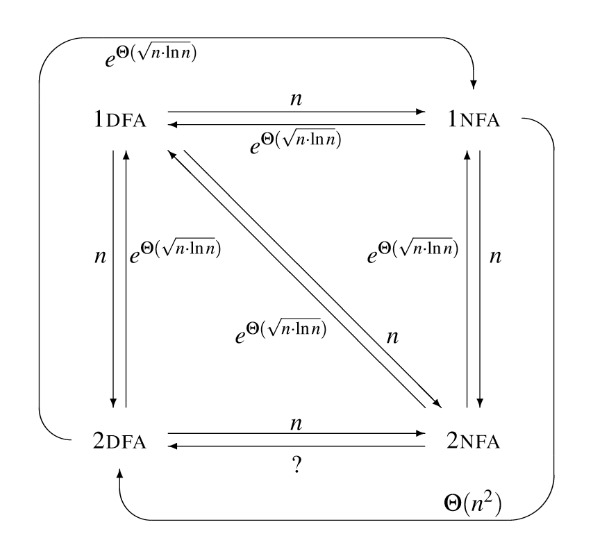
\includegraphics[width = 200 pt]{x}
\end{frame}
\begin{frame}
\frametitle{1nfa to 2dfa}
Lemma A: If gcd(a,b)=1, then the greatest number such that the equation $ax+by=c$ has no solutions in natural numbers is (a-1)(b-1)-1.\\
\medskip
Theorem:For each n there is a unary n-state 1nfa A such that each 2dfa recognizing L(A) requires $\Omega(n^2)$ states.\\
\medskip
Proof: Let L=$\{x| x= n x_1$+(n-1)$x_2$ for $x_1$, $x_2\in$N\}. L can be recognized by a lnfa
A with n states. A=(Q, $q_0$, E, F) is defined as follows: Q={$q_0$,..., $q_{n-l}$}, E =
\{($q_i$, $q_{i+1}$)$| i = 0,..., n- 1\}\cup {(q_1, q_3)}$ (the addition is mod n) and F = {$q_0$}. Let
m = max($\mathbb{N}$-L). By Lemma A, m = O($n^2$). Consider a 2dfa B recognizing L and its
computation on m. Suppose that, in all passes on m, B enters a cycle and let
$y_1$,...,$y_k$ be the lengths of these cycles. Then B would reject also m'=
m + lcm($y_1,.. , y_k$), which contradicts the fact that m' $\in$ L. Therefore, there is a pass.
of B on m without a cycle and the theorem follows. 

\end{frame}
\end{document}
